\chapter{Lecture}\label{part3:lec17} %%% 17
\markboth{\thechapter. Lecture}{\thechapter. Lecture}

We\pageoriginale continue our discussion of $p(n)$. Last time we
obtained 
$$
p(n) = \sum_{\substack{(h, k)=1\\0 \leq h < k \leq N}} \frac{i}{k^2}
e^{-2\pi i n h/k}
\int\limits^{\mathfrak{z}''_{hk}}_{\mathfrak{z}'_{hk}} f\left(e^{2 \pi i
  (\frac{h}{k} + \frac{\mathfrak{z}}{k^2})}\right) e^{2 \pi in
  \mathfrak{z}/k^2} d \mathfrak{z}
$$
$n$ is a fixed integer here, $n \gtreqless 0$ and $p(n)=0$ for $n< 0$;
and this will be of some use later, trivial as it sounds. $N$ is the
order of the Farey series. We have to deal with a complicated
integrand and we can foresee that there will be difficulties as we
approach the real axis. However, $f$ is closely related to $\eta$:
$$
\displaylines{\hfill 
  f(e^{2 \pi i \tau})= e^{\pi i \tau /12} (\eta (\tau))^{-1},\hfill \cr
  \text{since} \hfill f(x) = \frac{1}{\prod\limits^\infty_{m=1}(1-x^m)},
  \hfill \cr
  \hfill \eta(\tau) = e^{\pi i \tau/12} \prod^\infty_{m=1} (1- e^{2 \pi i m
    \tau}). \hfill }
$$

For us $\tau = \dfrac{h}{k} + \dfrac{i \mathfrak{z}}{k^2}$.

We can now use the modular transformation. We want to make $\im \tau$
large so that we obtain a big negative exponent. So we put $\tau' =
\dfrac{a \tau +b}{c \tau +d}, a, b, c, d$ being chosen in such a way
for small $\tau$, $\tau'$ becomes large. This is accomplished
by\pageoriginale\ taking $k \tau- h$ in the denominator; $k \tau -h=0$
when $z=0$ and close to zero when $z$ is close to the real axis. We
can therefore put $\tau'= \dfrac{a \tau + b}{k \tau -h}$ where $a$,
$b$ should be integers such that
$\left|\begin{smallmatrix} a & b \\ k &
-h\end{smallmatrix}\right|=1$. This gives $-ah -bk =1$ or $ah\equiv -1
\pmod{k}$. Take a solution of this congruence, say $h'$ i.e., choose
$h'$ in such a way that $h' h \equiv -1 \pmod{k}$, which is feasible
since $(h, k)= 1$. As soon as $h'$ is found, we can find $b$. Thus the
matrix of the transformation would be
$$
\begin{pmatrix} a & b\\ c & d \end{pmatrix}= 
\begin{pmatrix} h' & - \frac{hh'+1}{k}\\ k & -h \end{pmatrix}
$$ 

So we have found a suitable $\tau'$ for our purpose.
\begin{align*}
  \tau' & = \frac{h' \left( \dfrac{h}{k} + \dfrac{i
      \mathfrak{z}}{k^2}\right) - \dfrac{hh'+1}{k}}{k \left(
    \dfrac{h}{k} + \dfrac{i \mathfrak{z}}{k^2}\right) - h}\\
  & = \frac{h' \dfrac{i \mathfrak{z}}{k} -1}{i \mathfrak{z}}\\
  & = \frac{h'}{k} + \frac{i}{\mathfrak{z}}.
\end{align*}

If $z$ is small this is big.

Now recall the transformation formula for $\eta$: if $c> 0$, 
$$
\eta \left( \frac{a \tau + b}{c \tau+d}\right) = \epsilon \sqrt{\frac{c
    \tau+i}{i}} \eta ( \tau) 
$$

In\pageoriginale\ our case
\begin{align*}
  f(e^{2 \pi i \tau'}) & = e^{\pi i \tau' /12} (\eta (\tau'))^{-1}\\
  & = e^{\pi i \tau'/12} \epsilon^{-1} \left( \dfrac{c \tau
    +d}{i}\right)^{-1/2} (\eta(\tau))^{-1}\\
  & e^{\pi i \tau'/12} \epsilon^{-1} \left( \frac{c \tau
    +d}{i}\right)^{-1/2} e^{\pi i \tau/12} f(e^{2 \pi i \tau})
\end{align*}

And this is what we were after. Since
$$
c \tau +d = k \tau -h =k \left( \frac{h}{k} + \frac{i
  \mathfrak{z}}{k^2}\right) -h = \frac{i \mathfrak{z}}{k},
$$
this can be rewritten in the form:
\begin{align*}
  f(e^{2 \pi i \tau}) & = f(e^{2 \pi i \left(\frac{h}{k} + \frac{i
      \mathfrak{z}}{k^2}\right)})\\
  & = \epsilon e^{\dfrac{\pi i}{12}\left(\frac{h}{k} - \frac{h'}{k} \right)}
    e^{\dfrac{\pi i}{12} \left( \frac{i \mathfrak{z}}{k^2} -
      \dfrac{i}{\mathfrak{z}} \right)} \sqrt{\frac{\mathfrak{z}}{k}}
    f \left(e^{2 \pi i \left( \dfrac{h'}{k} + \dfrac{i}{\mathfrak{z}}\right)}\right)
\end{align*}
and there is no doubt about the square root - it is the principal
branch. We write
$$
\omega_{hk}= \epsilon e^{\dfrac{\pi i}{12} \left(\dfrac{h}{k} - \dfrac{h'}{k} \right)}
$$

So something mathematical has happened after all this long
preparation; and we can make some use of our previous knowledge. We
have
$$
  p(n) = \sideset{}{'}\sum_{o \leq h < k \leq N} \frac{i \omega_{hk}}{k^{5/2}}
  e^{- 2 \pi i n h/k}
  \int\limits_{\mathfrak{z}'_{hk}}^{\mathfrak{z}''_{hk}}
  e^{\frac{\pi}{12} \left( \frac{1}{\mathfrak{z}} -
    \frac{\mathfrak{z}}{k^2}\right)} \sqrt{\mathfrak{z}} f \left(e^{2 \pi i
  \left( \frac{h'}{k} + \frac{i}{\mathfrak{z}}\right)}\right) e^{2 \pi n
    \mathfrak{z}/k^2} d \mathfrak{z}  
$$
where\pageoriginale\ $\sum'$ denotes summation over $h$ and $k$, $(h,
k)=1$. Now what is the advantage we have got? Realise that
$$
f(x) = \sum^\infty_{n=0} p(n) x^n = 1+x + \cdots
$$

So for small $x$, $f(x)$ is close to 1. It will be a good
approximation for small arguments at least to replace $f(x)$ by 1. Let
us write
$$
\Psi_k (\mathfrak{z}) = \sqrt{\mathfrak{z}} e^{\frac{\pi}{2}
  \left(\frac{1}{\mathfrak{z}} -\frac{\mathfrak{z}}{k^2}  \right)} 
$$

Then 
\begin{multline*}
  p(n) = \sideset{}{'}\sum_{0 \leq h < k\leq N} \frac{i \omega_{hk}}{k^{5/2}} e^{-
  2 \pi in h/k} \int\limits^{\mathfrak{z}''_{hk}}_{\mathfrak{z}'_{hk}}
  e^{2\pi n \mathfrak{z}/k^2} \Psi_k (\mathfrak{z})
  d \mathfrak{z} +\\
  \sum_{o \leq h< k \leq N} \frac{ i \omega_{hk}}{k^{5/2}} e^{- 2 \pi
    i n h/k} \int\limits^{\mathfrak{z}''_{hk}}_{\mathfrak{z}'_{hk}}
  \Psi_k (\mathfrak{z}) \left\{ f(e^{2 \pi i \left( \frac{h'}{k} +
    \frac{i}{\mathfrak{z}}\right)}) -1 \right\}  e^{2 \pi n
    \mathfrak{z}/k^2} d \mathfrak{z}
\end{multline*}
where\pageoriginale\ the second term compensates for the mistake
committed on taking $f(x)=1$. The trick will be now to use the first
term as the main term and to use an estimate for the small
contribution from the second term. We have now to appraise
this. Writing $I_{hk}$ and $I^*_{hk}$ for the two integrals, we have
$$
p(n) = \sideset{}{'}\sum_{o \leq h < k \leq N} \frac{i \omega_{hk}}{k^{5/2}} e^{-
  2 \pi i n h/k} I_{hk} + \sideset{}{'}\sum_{o \leq h < k\leq N} \frac{i
  \omega_{hk}}{k^{5/2}} e^{- 2 \pi i n h/k} I^*_{hk}
$$

Here we stop for a moment and consider only $I^*_{hk}$ and see what
great advantage we got from our special path.
\begin{figure}[H]
  \centering{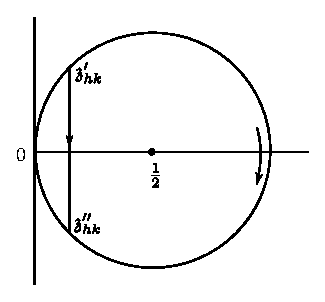
\includegraphics{vol2-figures/fig2.27.eps}}
\end{figure}

This is the arc of the circle $| z- \frac{1}{2}| = \frac{1}{2}$ from
$\mathfrak{z}'_{hk}$ to $\mathfrak{z}''_{hk}$ described
clockwise. Since $f(x)-1= \sum\limits^\infty_{m=1} p (\nu) x^\nu$, the
integrand in $I^*_{hk}$ is regular, and so for integration we can just
as well run across, along the chord from $\mathfrak{z}'_{hk}$ to
$\mathfrak{z}''_{hk}$. Let us see what happens on the chord. We have
\begin{align*}
  \left|\left( f(e^{2 \pi i h'/k- 2 \pi \mathfrak{z}})-1\right) \Psi_k
  (\mathfrak{z}) e^{2 \pi n \mathfrak{z}/k^2}\right| & =
  \left|\left(f(e^{2 \pi i h'/k- 2 \pi /\mathfrak{z}})-1 \right)
  \sqrt{\mathfrak{z}} e^{\frac{\pi}{12 \mathfrak{z}}- \frac{\pi
      \mathfrak{z}}{12 k^2}+ \frac{2 \pi n
      \mathfrak{z}}{k^2}}\right|\\
  & = \sqrt{\mathfrak{z}} e^{\mathscr{R}\frac{\pi}{12 \mathfrak{z}}}
    e^{\mathscr{R} \mathfrak{z} \frac{\pi}{k^2} (- \frac{1}{2} + 2n)}
    \times \left| \sum^\infty_{\nu=1} p(\nu) e^{(2 \pi i \frac{h'}{k}-
      \frac{2 \pi}{\mathfrak{z}})\nu }\right|  \\
    & \leq |\sqrt{\mathfrak{z}}| \sum^\infty_{\nu=1} p(\nu) e^{-
      \mathscr{R} \frac{1}{\mathfrak{z}} (2 \pi \nu - \frac{\pi}{12})}
    e^{\frac{\pi}{k^2} (- \frac{1}{12} + 2n) \mathscr{R}\mathfrak{z} }
\end{align*}

Let\pageoriginale\ us determine $\mathscr{R}\mathfrak{z}$ and
$\mathscr{R} \frac{1}{\mathfrak{z}}$ on the path of integration $o <
  \mathscr{R} \mathfrak{z} \leq 1$ on the chord. And
$\mathscr{R} \frac{1}{\mathfrak{z}} > 1$; for 
$$
\mathscr{R} \frac{1}{\mathfrak{z}} = \mathscr{R} \frac{1}{x+ iy} =
\frac{x}{x^2+ y^2},
$$
while the equation to the circle is $(x- \frac{1}{2})^2+y^2=
\frac{1}{4}$ or $x^2 + y^2=x$; the interior of the circle is $x^2 +
y^2< x$, and so $\mathscr{R} \frac{1}{\mathfrak{z}} \leq 1$, equality
on the circle.

$|\sqrt{\mathfrak{z}}|\leq $ the longer of the distances of
$\mathfrak{z}'_{hk}$, $\mathfrak{z}''_{hk}$ from 0. 

We\pageoriginale\ have already computed $\mathfrak{z}'_{hk}$ and
$\mathfrak{z}''_{hk}$:
\begin{align*}
  \mathfrak{z}'_{hk} & = \frac{k^2}{k_1^2 + k^2} + i \frac{k
    k_1}{k_1^2 + k^2},\\
  \mathfrak{z}''_{hk} & = \frac{k^2}{k_2^2 + k^2} + i \frac{k
    k_2}{k_2^2 + k^2}\\
  |\mathfrak{z}'_{hk}|^2 & = \frac{k^4 + k^2 k_1^2}{(k_1^2+ k^2)^2} =
    \frac{k^2}{k^2+ k_1^2} 
 \end{align*}

Now we wish to appraise this in a suitable way.
\begin{align*}
  2(k_1^2 + k^2) & = (k_1+ k^2)^2 + (k_1 - k)^2\\
  & \geq (k_1 +k)^2\\
  & \geq N^2,
\end{align*}
from our discussion of adjacent fractions. So
\begin{alignat*}{4}
  &&|\mathfrak{z}'_{hk}|^2 & \leq \frac{2k^2}{N^2}\\
  \text{or}&\hspace{2cm} & |\mathfrak{z}'_{hk}| & \leq \frac{\sqrt{2}
      \cdot k}{N};\hspace{3cm}\\
  \text{also} && |\mathfrak{z}''_{hk}| & \leq \frac{\sqrt{2}\cdot  k}{N}
\end{alignat*}

So\pageoriginale\ the inequality becomes
\begin{align*}
  \left| \left( f(e^{2 \pi i h'/k- 2 \pi
    /\mathfrak{z}})-1\right)\Psi_k (\mathfrak{z}) e^{2 \pi n
    \mathfrak{z}/k^2}\right| & \leq \sqrt[4]{2} \cdot
  \frac{k^{1/2}}{N^{1/2}} \sum^\infty_{\nu=1} p (\nu) e^{(2 \pi \nu -
    \pi/12)} e^{\pi (- \frac{1}{2} + 2/n 1)/k^2}\\
  & \leq C e^{2 \pi|n|} \frac{k^{1/2}}{N^{1/2}}
\end{align*}
where $C$ is independent of $\nu$, since the series
$\sum\limits^\infty_{\nu=1}p(\nu) e^{- (2 \pi \nu - \pi/12)}$ is
convergent. Since the length of the chord of integration $< 2 \sqrt{2}
\cdot k/(N+1)$m, we have
$$
\left| I^*_{hk} \right| < C_1 e^{2 \pi |n|} \frac{k^{3/2}}{N^{3/2}}
$$

Then 
\begin{align*}
  \left|  \sideset{}{'}\sum_{0 \leq h < k\leq N}  \frac{i \omega_{hk}}{k^{5/2}}
  e^{- 2 \pi n h/k} I^*_{hk} \right| & \leq C_1 e^{2 \pi |n|} \sideset{}{'}\sum_{0
    \leq h < k \leq N} \frac{1}{k N^{3/2}}\\
  & \leq C_1 e^{2 \pi |n|} \sum_{0 < k \leq N} \frac{1}{N^{3/2}},
\end{align*}

Since\pageoriginale\ the summation is over $h < k$ with $(h, k)=1$,
so that there are only $\varphi (k)$ terms and this is $\leq k$. So
the last expression is
$$
C_1 e^{2 \pi |n|} N^{-1/2}
$$

Hence
$$
p(n) = \sum_{o \leq h< k \leq N} \frac{i \omega_{hk}}{k^{5/2}} e^{-
  2\pi in h/k} I_{hk} + R_N
$$
where
$$
|R_N| < C_1 e^{2 \pi |n| N^{- 1/2}}
$$

